\documentclass[a4paper,12]{article}

\usepackage{listings}
\usepackage{booktabs}
\usepackage{amsmath}
\usepackage{a4wide}
\usepackage{tikz}
\usetikzlibrary{shapes, calc, shapes, arrows}
\usepackage{relsize}
\usepackage{subcaption}
\usepackage{amssymb}
\usepackage{enumerate}
\usepackage{array}
\usepackage{mathrsfs}
\usepackage{graphicx}
\usepackage{algorithm2e}
%\usepackage[utf8]{inputenc}
\usepackage[T1]{fontenc}
\usepackage{pxfonts}
\usepackage{cite}
\usepackage{hyperref}
\usepackage{abstract}

\lstset{basicstyle=\ttfamily,
literate=
  {á}{{\'a}}1 {é}{{\'e}}1 {í}{{\'i}}1 {ó}{{\'o}}1 {ú}{{\'u}}1
  {Á}{{\'A}}1 {É}{{\'E}}1 {Í}{{\'I}}1 {Ó}{{\'O}}1 {Ú}{{\'U}}1
  {à}{{\`a}}1 {è}{{\`e}}1 {ì}{{\`i}}1 {ò}{{\`o}}1 {ù}{{\`u}}1
  {À}{{\`A}}1 {È}{{\'E}}1 {Ì}{{\`I}}1 {Ò}{{\`O}}1 {Ù}{{\`U}}1
  {ä}{{\"a}}1 {ë}{{\"e}}1 {ï}{{\"i}}1 {ö}{{\"o}}1 {ü}{{\"u}}1
  {Ä}{{\"A}}1 {Ë}{{\"E}}1 {Ï}{{\"I}}1 {Ö}{{\"O}}1 {Ü}{{\"U}}1
  {â}{{\^a}}1 {ê}{{\^e}}1 {î}{{\^i}}1 {ô}{{\^o}}1 {û}{{\^u}}1
  {Â}{{\^A}}1 {Ê}{{\^E}}1 {Î}{{\^I}}1 {Ô}{{\^O}}1 {Û}{{\^U}}1
  {œ}{{\oe}}1 {Œ}{{\OE}}1 {æ}{{\ae}}1 {Æ}{{\AE}}1 {ß}{{\ss}}1
  {ű}{{\H{u}}}1 {Ű}{{\H{U}}}1 {ő}{{\H{o}}}1 {Ő}{{\H{O}}}1
  {ç}{{\c c}}1 {Ç}{{\c C}}1 {ø}{{\o}}1 {å}{{\r a}}1 {Å}{{\r A}}1
  {€}{{\euro}}1 {£}{{\pounds}}1 {«}{{\guillemotleft}}1
  {»}{{\guillemotright}}1 {ñ}{{\~n}}1 {Ñ}{{\~N}}1 {¿}{{?`}}1
}

% Disable text indent for paragraph
\setlength{\parindent}{0pt}

\title{Artificual Neural Networks \& Deep QLearning}
\author{Jan Vincent Hoffbauer\\
jan.hoffbauer@rwth-aachen.de }
\date{\today}

\begin{document}

\maketitle
~\\
\\
\\

\begin{abstract}
In this paper I describe Artificial Neural Networks and Deep Q-Learning. I briefly sumarize the mathematical background and present usage examples of these algorithms. Furthermore I apply them to practical examples. 
\end{abstract}
  
\newpage
\tableofcontents
\newpage

% List all citations
\nocite{*}

% Introduction
\section{Introduction}
Machine learning has become an important of computer science. Since the development of the internet, huge amounts of data are becoming available. The machine learning algorithms presented in this paper can derive knowledge from such data. For example, artificial neural networks can be used to recognize faces on images or predict trends in the stock market. 
\\
\\
In this paper I will first introduce, how machine learning models can be evaluated. Then I will introduce artificial neural networks and Deep Q-Learning, to give the reader a basic overview about different machine learning technologies. 


\section{Evaluating Models}

% Overfitting
% Seperate training and test data
% k-fold cross validation

It is neccessary to evaluate the performance of machine learning models. To evaluate a model, it is common to use the output error on a certain dataset to evaluate the performance of the model. In most cases, the initial dataset is split into a training set and a test set. The training set is used to train the model, the test set is used to evaluate the model. It is important to not use the same dataset for training and testing, because this contains the risk of the model simply memorizing all single entries of the data set, which is called overfitting. 
\\
\\
To enhance the data usage, a method called $k$-fold cross validation can be used. The idea is to do multiple training and evaluation rounds by selecting different training and test sets each round. The dataset is split into $k$ equally sized subsets. Then $k$ rounds of training and evaluating are done. Each round $1/k$ of the data is used as test set, the remaining data is used to train the model. The average score of the data should give a better estimate about the models quality. Typical values for $k$ are $k=5$ or $k=10$.

\section{Artificial Neural Networks}
          
Artificial Neural Networks are a machine learning model inspired by the human brain. The basic idea behind artificial neural networks is to model the electrochemical activity of single brain cells, called neurons. Figure \ref{fig:neuron} shows the mathematical model of single artificial neuron.
\\
\tikzstyle{inputNode}=[draw,circle,minimum size=10pt,inner sep=0pt]
\tikzstyle{stateTransition}=[->, thick]
\begin{figure}[h]
\centering
\begin{tikzpicture}
	\node[draw,circle,minimum size=35pt,inner sep=0pt] (x) at (0,0) {$\mathlarger{\mathlarger{\Sigma \textbf{   } g}}$};

	\node (x0) at (-3, 1.5)  {$\tiny a_0$};
	\node (xi)  at (-3, 0)     {$\tiny a_i$};
	\node (xn) at (-3, -1.5) {$\tiny a_n$};

	\draw[stateTransition] (x0) to node [above=-3, sloped, sloped, midway] {$w_{0, j}$} (x);
	\draw[stateTransition] (xi)  to node [above=-2] {$w_{i,j}$} (x);
	\draw[stateTransition] (xn) to node [above=-3, sloped, midway] {$w_{n, j}$} (x);
	
	\node (dots) at (-3,  0.85) {$\vdots$};
	\node (dots) at (-3, -0.55) {$\vdots$};
	
	\draw[stateTransition] (x) -- (3,0) node [midway,above=-0.1cm] {$ \mathsmaller{a_j = g(in_j)}$};

	\draw[dashed] (0,-0.50) -- (0,0.50);
\end{tikzpicture}
\caption{Schematic description of an artificial neuron}
\label{fig:neuron}
\end{figure}

A neural network is composed of several neurons. These neurons are connected by directed links, called synapis. The synapsis propagate the activation from neuron $i$ to neuron $j$. It has an associated weight called $w_{i,j}$, which denotes the strength of the synapsis. 
\\
\\
It is common to add an additonal neuron to the input neurons of each neuron. This neuron is called the bias neuron and has a constant activation, allowing to shift the neurons output by a certain value. This is often important for successfull learning. The bias neuron of neuron $j$ is denoted by $bias_j$
\\
\\
A neurons weighted input is calculated the following way:

\begin{equation*}
in_j = bias_j + \sum\limits_{i \in Input_j} w_{i,j} a_i.
\end{equation*}

To calculate the activation of the neuron, the activation function $g$ is applied to the weighted input and the bias neuron:

\begin{equation*}
a_j = g(in_j).
\end{equation*}
\\
Typical activation functions are the hyperbolic tangent or sigmoid function. An important property of the activation function is to provide a smooth transition as the input value changes. Furthermore it has to be derivable, to allow application of the backpropagation algortihm, I will introduce later. 


\subsection{Structure} 

There are two fundamentally distinct ways to connect the neurons in a neural network. On the one hand there are feedforward networks, on the other hand there are recurrent networks.
\\
\\
In feedforward networks all connections are directed in the same direction. This makes the network an acyclic graph and the activations following a certain direction. Due to the fact, that a neurons input is only affected by the preceeding neurons and the neurons output only affects the succeeding neurons, there are no loops. Thus the neuronal network has no internal state and represents a function of the input. 
\\
\\
Recurrent networks allow for such loops. Thus the output of certain neurons can be used as input to these neurons again. This makes the networks behavior far more complex to understand, but also allows the neuronal network to preserve an internal state. That allows the neuron to have some kind of short term memory.
\\
\\
In this article I will focus on feedforward neuronal networks. It is common to arrange the neurons of feedforward networks in so called layers. These layers are used to bundle a set of neurons. The layers are ordered in the neural network and each layer uses the preceeding layer as input. The first layer is called the input layer and the last layer is called the output layer. The layers between the input and output layers are called hidden layers. Neural networks without hidden layers are called perceptron networks and neural networks with multiple hidden layers are called multilayer networks. 
\\
\begin{figure}[h]
	\centering

	\tikzstyle{neuron}=[draw, circle, minimum size=19pt, inner sep=0pt]

	\begin{subfigure}{.3333\textwidth}
		\centering
		\begin{tikzpicture}
			\node[neuron] (n1) at (0,0)    {1};
			\node[neuron] (n2) at (0,1)    {2};
			\node[neuron] (nout) at (1.5,0.5) {out};
			
			\draw [->] (n1) -- (nout);
			\draw [->] (n2) -- (nout);
			
			\node (x1) at (-1, 0) {$x_1$};
			\node (x2) at (-1, 1) {$x_2$};
			\draw [->] (x1) -- (n1);
			\draw [->] (x2) -- (n2);
			
		\end{tikzpicture}
    	 \caption{}
    \end{subfigure}%    
    % 
    \begin{subfigure}{.3333\textwidth}
		\centering
		\begin{tikzpicture}
			\node[neuron] (n1) at (0,0)    {1};
			\node[neuron] (n2) at (0,1)    {2};
			\node[neuron] (n3) at (1.5,0)    {3};
			\node[neuron] (n4) at (1.5,1)    {4};
			\node[neuron] (nout) at (3,0.5) {out};
			
			\draw [->] (n1) -- (n3);
			\draw [->] (n1) -- (n4);
			\draw [->] (n2) -- (n3);
			\draw [->] (n2) -- (n4);
			\draw [->] (n3) -- (nout);
			\draw [->] (n4) -- (nout);
			
			\node (x1) at (-1, 0) {$x_1$};
			\node (x2) at (-1, 1) {$x_2$};
			\draw [->] (x1) -- (n1);
			\draw [->] (x2) -- (n2);
			
		\end{tikzpicture}
        \caption{}
	\end{subfigure}%
	
	\caption{Shown are two network architectures for approximating the XOR-function. (a) Shows a perceptron network. (b) Shows a feedforward network with an hidden layer of two neurons}
	\label{fig:xor}
\end{figure}

The networks shown in Figure \ref{fig:xor} can be trained to compute the XOR-function. In Table \ref{tab:xor} you can see the truth table of the XOR-function and the outputs of the two displayed networks.
\\
\begin{table}[h]
  \centering
  \begin{tabular}[c]{cccrr}
    \hline
    \multicolumn{3}{l}{XOR data} 		& \multicolumn{2}{l}{network output}	\\
    \hline
    $x_1$ 		& $x_2$		& $y$	 		& 	perceptron 	& 	multilayer 	\\
    \hline
    0 				& 0 				& 0				& .50				& .00				\\
    0 				& 1 				& 1				& .50 				& .99 				\\
    1 				& 0 				& 1				& .50 				& .99 				\\
    1 				& 1 				& 0				& .50 				& .00 				\\
    \hline
  \end{tabular}
  \caption{output of different networks on XOR data after 50000 training epochs}
  \label{tab:xor}
  
\end{table}

As you can see, the perceptron network is not able to compute the XOR-function. The multilayer network on the other hand can compute the XOR-function easily. The reason for that result is, that an perceptron can only compute linearly seperable functions. To compute more complex functions more layers are required. Actually, it can be shown, that a feedforward neural network with one sufficiently large hidden layer can compute any continuous function of the inputs with arbitrary accuracy.  An feedforward network with two layers can compute even discountinuous functions. 


\subsection{Learning}

The natural question arises, how to train a feedforward neural network. In the following I will introduce the backpropagation algorithm, which can be used to train such a network. 
\\
\\
Interpreting the feedforward neural network as a vector function helps understanding the backpropagation algorithm. Each neuron is interpreted as component of the vector, representing its layer. To calculate the output of such a neural network, the activations of each layers neurons are computed consecutively, as shown in the following algorithm: 
\\
\\
\begin{algorithm}[H]
	\KwData{ input vector $x$ }
	\KwResult{ activations $a_i$ for all neurons }
	\For{ neuron $j$ in input layer } {
		$a_j \leftarrow x_j $
	}
	\For{ $l=2$ to layer count } {
		\For {neuron $j$ of neurons in $l$ } {
			$a_j \leftarrow g(\sum\limits_{i \in Input_j} w_{i,j} a_i + bias_j)$
		}
	}
	\For{ neuron $k$ in output layer }  {
		$h_k \leftarrow a_k$	
	}
\end{algorithm}
~\\
After the output vector $h$ of the network is calculated for a certain input, the networks output and the target output $y$ can be compared. The output error is calculated using an error function. After the output error is calculated, it is neccessary to compute the error of the neurons in the previous layers. This is done by backpropagating the error. 
\\
\\
It is common to use squared error as error function, which is shown in the following:

\begin{equation*}
L_2 = (y_k - h_k)^2.
\end{equation*}
\\
To reduce the error $L_2$ of the networks output, we can change $h_k$. To change $h_k$, we can thus change $in_k$, because $h_k = g(in_k)$. The amount about which to change $in_k$ can be obtained by deriving $L_2$ with respect to $in_k$: 

\begin{equation*}
\frac{ \delta L_2 }{ \delta in_k }    =    \frac{ \delta ((y_k - h_k)^2) }{ \delta in_k }     =      \frac{ \delta (y_k - g(in_k)) }{ \delta in_k }  *  2 * (y_k - g(in_k) )   =   g'(in_k) * 2 * (y_k - g(in_k)).
\end{equation*}
\\
By leaving out the $2$ as constant factor and defining $Err_k = y_k - g(in_k)$ , we define a modified error:

\begin{equation}
\label{eq:bp:errout}
\Delta_k = Err_k * g'(in_k).
\end{equation}
\\
This error will later be used, to compute the weight update of the network. If the network contains hidden layers, it is neccessary to compute a similar measure of error for the hidden layer neurons too. To do this, we can backpropagate the error to these neurons. Neuron $j$ affects the error $\Delta_k$ of each neuron $k$ it connects to as input neuron by a certain amount, scaled by the weight $w_{j,k}$ from $j$ to $k$. The idea is to add up the error $j$ produces: 

\begin{equation}
\label{eq:bp:errhid}
\Delta j = g'(in_j) * \sum\limits_k w_{j,k} * \Delta_k.
\end{equation}

As the error $\Delta_j$ for every neuron in the network is computed, the error can be used to update the weights of every synapsis. The weight update is aimed to reduce the general error $L_2$. To update the weights, the following rule is used:

\begin{equation}
\label{eq:bp:wupd}
w_{i,j} \leftarrow w_{i,j} + \alpha * a_i * \Delta_j.
\end{equation}

Here $\alpha$ is the learning rate, determining how much to change the weights each weight update. To understand the weight update rule, it is important to know, that $\frac{ \delta L_2 }{ \delta w_{i,j} } = -a_i * \Delta_j$, both for the output and hidden layers. Because of this, to reduce the output error by changing $w_{i,j}$, the weight $w_{i,j}$ has to be changed by $\frac{ \delta L_2 }{ \delta w_{i,j} }$. Thus the weight update rule changes each weight in a way, so that the error is reduced. 
\\
\\
To update the biases, similar considerations are applied. Due to $\frac{ \delta L_2 }{ \delta bias_i } = \Delta_j$, the bias update rule becomes: 

\begin{equation}
\label{eq:bp:bupd}
bias_i \leftarrow \alpha * \Delta_i.
\end{equation}

The final algorithm follows the following steps for each training example: 
\begin{itemize}
\item Do feedforward pass	
\item Calculate output errors using Equation \ref{eq:bp:errout}
\item Backpropagate errors using Equation \ref{eq:bp:errhid}
\item Do weight update using Equation \ref{eq:bp:wupd} and bias update using Equation \ref{eq:bp:bupd}
\end{itemize}
~\\ 
The actual algorithm becomes:
\\
\\
\begin{algorithm}[H]
	\KwData{ set of examples, each containing input $x$ and target $y$ }
	\KwResult{ activations $a_i$ for all neurons }
	
	do forward step, calculating $in_j$, $a_j$ for each neuron $j$\\
	\For{ neuron $k$ in output layer } {
		$\Delta_k \leftarrow (y_k - a_k) * g'(in_k)$
	}
	\For{ $l=2$ to $L$ } {
		\For {neuron $i$ of neurons in $l$ } {
			$ \Delta_i \leftarrow g'(in_i) * \sum_j w_{i,j} * \Delta_j$
		}
	}
	\For{ weight $w_{i,j}$ of each synapsis in network } {
		$ w{i,j} \leftarrow w_{i,j} + \alpha * a_i * \Delta_j $
	}
	\For { neuron $i$ in network } {
		$ bias_i \leftarrow  \alpha * \Delta_i $
	}
\end{algorithm}
~\\
 
 
\subsection{Practical usage of Neural Networks}

% ANN on iris versicolor dataset 
% Describe problem: 3 classes, measured data, data source, 150 entries
% Describe class encoding
% Describe nn 4,8,3 sigmoid
% Describe K-Folding 3
% Describe result, accuracy def

To describe the practical usage of neural networks, I apply a feedforward neural network to the Iris data set. The Iris data set is a well studied data set in the area of machine learning. It can be obtained from the UCI Machine Learning Repository \cite{UCI}. The dataset contains 150 entries, each denoting several attributes of an Iris plant and its classification. The attributes are sepal length in cm, sepal width in cm, petal length in cm and petal width in cm. The possible classifications are Iris Setosa, Iris Versicolour and Iris Virginica. My goal is to train a neural network to classify each entry by using the attributes as input. 
\\
\\
The classes are encoded using one-hot encoding. For this classification problem this leads to the following encoding shown in Table \ref{tab:iris_encoding}.

\begin{table}[tb]
  \centering
  \begin{tabular}[c]{lc}
    \hline
    classification			& $y$ 					\\
    \hline
    Iris Setosa 				& $(1, 0, 0)$		\\
    Iris Versicolour 		& $(0, 1, 0)$		\\
    Iris Virginica 			& $(0, 0, 1)$		\\
    \hline
  \end{tabular}
  \caption{one-hot encoding of Iris dataset}
  \label{tab:iris_encoding}
\end{table}


As model, I use a feedforward neural network with 4 input neurons, one hidden layer of 8 neurons and an output layer of 3 neurons. As activation function I use the $sigmoid$ function. 
\\
\\
To evaluate the network, k-fold cross validation with $k=5$ is used. In addition to the output error I also calculate the accuracy of the network. The accuracy determines, how much of the entries from the test set are classified correct. An entry is considered correctly classified, if for every output neuron $k$: 

\begin{equation*}
y_k =\lfloor h_k \rceil.
\end{equation*}
\\
The accuracy is defined as the percentage of correctly classified entries:

\begin{equation*}
accuracy = \frac{ num_{correct} }{ num_{test} }.
\end{equation*}
\\
The results of my implementation are shown in the below table: 
\\
\\
\begin{table}[h]
  \centering
  \begin{tabular}[c]{crr}
    \hline
    round			& error						& accuracy (\%) 		\\
    \hline
    1					& 0.030					& 100.00					\\
    2					& 0.049					& 96.67					\\
    3					& 0.057					& 93.33					\\
    4					& 0.029					& 100.00					\\
    5					& 0.037					& 100.00					\\
    \hline
    average		& 0.040					& 98.00					\\
    \hline
  \end{tabular}
  \caption{Evaluation results classifier to Iris dataset}
  \label{tab:kfold}
\end{table}
\\
As you can see, my implementation archieved an average accuracy of $98\%$, which is quite typical for this data set. In the table I show a sample output of the trained neural network:
\\
\\
\begin{table}[h]
  \centering
  \begin{tabular}[c]{cccr}
    \hline
    $x$								& output			& target			& error		\\
    \hline
    $(5.5, 2.4, 3.7, 1.0)$ 	& $(0, 1, 0)$ 	& $(0, 1, 0)$  	& $0.00$	\\
    $(5.0, 3.4, 1.5, 0.2)$ 	& $(0, 0, 1)$	& $(0, 0, 1)$   & $0.00$	\\
    $(6.0, 2.9, 4.5, 1.5)$ 	& $(0, 1, 0)$	& $(0, 1, 0)$   & $0.00$	\\
    $(6.0, 2.7, 5.1, 1.6)$ 	& $(1, 0, 0)$ 	& $(0, 1, 0)$ 	& $0.67$	\\
    $(5.8, 2.7, 5.1, 1.9)$ 	& $(1, 0, 0)$ 	& $(1, 0, 0)$   & $0.00$	\\
    \hline
  \end{tabular}
  \caption{Sample output on Iris dataset}
  \label{tab:iris_example}
\end{table}


\section{Deep Q-Learning}

\subsection{Introduction}

\begin{figure}[h]
	\centering
	
	\begin{subfigure}{.3333\textwidth}
		\centering
		\includegraphics[width=4cm]{cartpole.png}
		\caption{}
		\label{fig:cartpole}
    \end{subfigure}%    
    % 
    \begin{subfigure}{.3333\textwidth}
		\centering
		\includegraphics[height=2.5cm]{breakout.png}
		\caption{}
		\label{fig:cartpole}
	\end{subfigure}%
	
	\caption{Shown are two examples of environments, Deep Q-Learning can be used for. (a) Cartpole (b) Atari Breakout game}
	\label{fig:examples}
\end{figure}

The question arises, how to train an agent in a complex environment, that reacts to the agents actions. Examples for such an environment are games like Atari-Breakout or the cartpole example.
\\
\\
It is not easily possible to provide training data for decision making, because the decision and the result may be remote in time from each other. One way to address such an problem is Deep Q-Learning. This algorithm was proposed in 2013 by Google DeepMind \cite{DQN} and has successfully been applied to several Atari-Games. Deep Q-Learning is an extension of Q-Learning. To introduce Deep Q-Learning I will first provide an formalisation of such an environment, then introduce Q-Learning and extend it to Deep Q-Learning. 
\\
\\
To apply this algorithm, the world is modelled as Markov-Decision-Process. The environment is represented as state vector $s_i$. Considering the state $s_i$ the agent can choose a certain action $a_i$. Actions transform the state and may lead to a reward $r_i$. A Markov-Decision-Process may be stochastic, denoting that the state resulting from taking a certain action in a certain state is not deterministic. The set of states, corresponding actions and rules for transitioning between these states and for getting rewards form the Markov-Decision-Process. 
\\
\begin{figure}
	\centering
	\begin {tikzpicture}[auto]
		\node[draw, circle] (agent) at (0,1.5) [] {agent};
		\node[draw, rounded corners, minimum width=40pt, minimum height = 20pt] (environment) at (0,0) {environment};
		\path [draw, ->] (environment) 	to [out=190, 	 in=180] 				node {state, reward} 		(agent);
		\path [draw, ->] (agent) 				to [out=350,     in=0] 					node {action} 					(environment);
	\end{tikzpicture}
    
	\caption{Reinforcement Learning problem}
	\label{fig:refprob}
\end{figure}


One episode of a Markov-Decision-Process leads to a chain of consecutive states, actions and rewards: 
$s_0, a_0, r_0,  s_1, a_1, r_1,  s_2, a_2, r_2, ..., s_n, a_n, r_n, $
\\
\\
The expected value of an action can not be measured by simply summing up all expected future rewards, because a Markov-Decision-Process is stochastic. Thus it can not be guaranteed, that the states visited during one episode are always the same. The uncertainity, that the expected reward and the actual reward diverge grows, the further the decision is away in time. An appropriate tool to measure the value of an action is expected discounted future reward. Here $\gamma$ is called discount factor, denoting how much reward \textit{discounts} over time.

\begin{equation*}
R_t = r_t + \gamma * r_{t+1}  +  \gamma^2 * r_{t+2}   +   ...   +    \gamma^{n-t} * r_{t+n}. 
\end{equation*}


% Introduce Q-Learning (Q-Table, Policy, Bellman Equation)
\subsection{Q-Learning}

Q-Learning is an algorithm to learn a policy to determine the best action for every state. A function $Q(s, a)$ is defined. This function will be trained to represent the discounted reward for every state action-pair. Using this function the policy $\pi$ determines the best action for every given state, by choosing the action with the expected highest discounted reward:

\begin{equation*}
\pi(s) = argmax_a Q(s, a).
\end{equation*}
\\
To train the $Q$ function, the algorithm can iteratively consider multiple transitions in the Markov-Decision-Process $(s, a, r, s')$ and update the Q-function acording to the Bellman-Equation:

\begin{equation*}
Q(s, a) = r + \gamma * max_{a'}Q(s', a').
\end{equation*}
\\
The idea behind this equation is, that the $Q$-Fuction will hold the true expected future discounted reward, if it has been updated with enough transitions. 
\\
\\
The final algorithm lets the agent learn in its environment by executing multiple actions and observing the transitions: 
\\
\\
\begin{algorithm}[H]
	\KwData{ rules for Markov decision process, number of training episodes $E$, learning rate $\alpha$ }
	\KwResult{ trained Q-Table }
	\For{ $i$ from $1$ to $E$ } {
		$ s \leftarrow $ observe initial state \\
		\While{ not terminated } {
			$ a \leftarrow \pi(s) $	\\
			$ r, s' \leftarrow$ carry out a and observe reward and new state 		\\
			\eIf { environment not terminated } {
				$ Q(s, a) = Q(s', a') + \alpha * (r + \gamma * max_{a'}) $
			} {
				$ Q(s, a) \leftarrow r $
			}
			$ s \leftarrow s' $
		}
	}
\end{algorithm}
~\\
\\
Applying this algorithm to the cartpole example may lead to the following exemplary Q-Table. The state vector of the cartpole example contains of the cartpoles current x position, the previous x position, the current pole angle, the previous pole angle.: 
\\
\begin{table}[h]
  \centering
  \begin{tabular}[c]{llc}
    \hline
    $s_i$												& $a$ 		& 	$Q(s, a)$				\\
    \hline
    $(2.32, 2.29, 0.14, 0.16)$ 				& Right 	& $0.132 $  			\\
    $(1.21, 1.24, 0.19, 0.11,)$ 			& Left 	& $0.442$   				\\
    $(0.03, 0.12, 1.47, 1.59)$ 				& Right 	& $0.842$   				\\
    ... 																& ...			& ... 				\\
    \hline
  \end{tabular}
  \caption{Extract of exemplary Q-Table}
  \label{tab:qtable}
\end{table}


\subsection{Deep Q-Learning}

Applying Q-Learning to complex states like the raw graphical input of an Atari-Game is nearly impossible, because the number of possible states and thus the entries to the Q-Table grows very quick. One solution to this problem is using an neural network, called Q-Network, to approximate the Q-Table. Neural networks have proven to work very well on highly structured data, like image data. In the original paper a neural network has been used to approximate the Q-Table. The algorithm achieved human level results on several Atari-Games. In the following I will introduce the Deep Q-Learning algorithm and the show practical results applying it to the Breakout-Game and cartpole example. 

\subsubsection{Q-Network}

The Q-Network takes the state vector as input and outputs expected discounted future reward for every possible action. The network structure is shown in the following figure:
\\
\begin{figure}[h]
	\centering

	\tikzstyle{input}=[draw, circle, minimum size=19pt, inner sep=0pt]

	\centering
	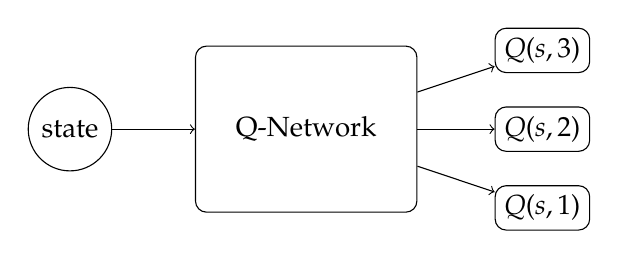
\begin{tikzpicture}
	
		\node[draw, circle, minimum size=20pt] (state) at (0,0)    {state};
		\node[draw, rounded corners, minimum width=80pt, minimum height=60pt] (qnet) at (3,0) 	{Q-Network};
		
		\node[draw, rounded corners] (q1) at (6,-1) 		{ $Q(s, 1)$ };
		\node[draw, rounded corners] (q2) at (6,0) 		{ $Q(s, 2)$ };
		\node[draw, rounded corners] (q3) at (6,1) 		{ $Q(s, 3)$ };
		
		\draw [->] (state) -- (qnet);
		\draw [->] (qnet) -- (q1);
		\draw [->] (qnet) -- (q2);
		\draw [->] (qnet) -- (q3);
			
	\end{tikzpicture}
	\caption{Input and Output structure of Q-Network}
	\label{fig:qnet}
\end{figure}

Given an transition $(s, a, r, s')$ the Q-Network is trained to predict the new value for the action: 

\begin{equation*}
y = r + \gamma * max_{a'}Q(s', a').
\end{equation*}
\\
The network is trained doing a backpropagation step on $(y - Q(s, a))^2$.

\subsubsection{Experience Replay}

To achieve better training results the visited transitions are stored in the so called replay-memory. Every step a batch of this replay-memory is sampled. The Q-Network is then trained using this batch. This approach results in better training results, because each step is potentially used in multiple weight updates. Furthermore multiple consecutive transitions may have strong correlation. Randomizing the samples breaks these correlations and avoids the agent to get stuck in a local minimum. If the correct action for the agent may be to turn right for a long period of time the training data will be dominated by such examples. By sampling the transitions from the replay memory, these transitions are spread over multiple batch updates.  

\subsubsection{Exploration}

In Deep Q-Learning the actions choosen initially are random, because the Q-Table is initialized randomly. Thus the agent may stuck in a certain local minimum. To avoid this, the agent "explores" random transitions. In every step with a probability $\epsilon$ the agent chooses a random action. It is common to reduce $\epsilon$ with every training episode to let the agent optimize its strategy after exploration. 

\subsubsection{Final Algorithm}

The final algorithm becomes: 
\\
\\
\begin{algorithm}[H]
	\KwData{ rules for Markov decision process, number of training episodes $E$ }
	\KwResult{ trained Q-Network }

	initialize replay memory $R$ to capacity $M$		\\
	initialize Q-Network $Q$ with random weights		\\	
	
	\For{ $i$ from $1$ to $E$ } {
		$ s \leftarrow $ observe initial state					\\
		\While{ not terminated } {
			With probability $\epsilon$ select random action $a$ 		\\
			Otherwise select action $a$ by executing $\pi(s)$			\\
			$ r, s' \leftarrow $ Carry out a and observe reward and new state	\\
			Sample random minibatch of transitions from $R$			\\
			\For {every transition $(s_i, a_i, r_i, s'_i)$ in minibatch} {
				\eIf {environment not terminated } { 
					$y_i \leftarrow r + \gamma * max_{a_i'}Q(s_i', a_i')$
				 } {
				 	$y_i \leftarrow r_i$
				 }
				 Train Q-Network using $(y_i - Q(s_i, a_i))^2$  \\
			}
		}
	}
\end{algorithm}

\subsection{Practical Results}

\subsubsection{Atari Games}

In the original paper \cite{DQN} Deep Q-Learning was used to play several Atari-Games. The games were emulated by an Atari game emulator which displays the games as 210x160 RGB images at 60 Hz. It is not possible to derive the full game state from one image, because motion information can not be derived. Thus a sequence of consecutive images have to be stacked, to model one state of the Markov decision process. Additionally the images are bascially downscaled to achieve better performance. As Q-Network a convolutional network, consisting of 3 convolutional layers and 2 fully connected layers, is used. Convolutional networks are a special kind of neural networks used for image processing. Convolutional networks used by Deep Q-Learning are referred to as Deep Q-Networks. 
\\
\\
The authors implementation of the Deep Q-Learning algorithm was tested on 7 Atari games. They report, that their method achieves better performance than an expert human player on Breakout, Enduro and Pong and it achieves close to human performance on Beam Rider. The same network architecture and hyperparameters were used across these games. 
\\

\begin{table}[h]
  \centering
  \begin{tabular}[c]{lccccccc}
    \hline
    						& B. Rider 		& Breakout 		& Enduro 	& Pong 	& Q*bert 		& Seaquest 	& S. Invaders			\\
    \hline
    Human			& 7456				& 31					& 368			& -3			& 18900		& 28010			& 3690						\\
    DQN				& 4092				& 168				& 470			& 20			& 1952			& 1705				& 581						\\
    DQN Best		& 5184				& 225				& 661			& 21			& 4500			& 1740				& 1075						\\
    \hline
  \end{tabular}
  \caption{ \cite{DQN} 
  					The upper table compares average total reward for Deep Q-Learning to an expert human player. 
  					The row DQN Best shows the single best performing episode of Deep Q-Learning. }
  \label{tab:comparison}
\end{table}


\subsubsection{Cartpole Example}

% Architecture + Preprocessing + ANN
% Results

I applied my implementation of Deep Q-Learning to the cartpole example. In this 2 dimensional example a pole is attached to a cart, which moves along a track. The goal is to keep the pole standing upright, by moving the cart. An image of the cartpole is shown in Figure \ref{fig:cartpole}.
\\
\\
To simulate the cartpole I used the Python OpenAI Gym, a powerfull toolkit to work with reinforcement learning. My implementation of Deep Q-Learning was written in Python. The Deep Learning library Keras was used to implement the Q-Network. To apply Deep Q-Learning the cartpole model is modelled as Markov decision process. Each state consists of the cartpoles current x position, the previous x position, the current pole angle, the previous pole angle. As Q-Network a feedforward network, consisting of 3 layers with 24 neurons each, was used. As activation function $tanh$ was used. To train the agent minibatches of size 32 were sampled from a replay memory of size 2000, with $\epsilon$ annealed linearly from 1.0 to 0.0 and fixed at 0.0 thereafter. 
\\
\\
I capped the number of possible steps in the cartpole example to 2000 steps, to avoid the training process getting stuck in an infinite loop. The observed average number of steps during 2000 training episodes is shown in Figure \ref{fig:cartpole_result}
\\
\begin{figure}
	\centering
	\includegraphics[width=10cm]{results-cartpole-avg10-2017steps.png}
	\caption{Deep Q-Learning training results for cartpole example}
	\label{fig:cartpole_result}
\end{figure}

As you can see the number of steps does not converge to the maximum of 1000 in a stable way, but the number of steps per episode increases and reaches the maximum several times. As the authors of the original payper state, a problem with Deep Q-Learning is, that small changes to the Q-Network may lead to big changes in the actions taken. 




\section{Conclusion and Outlook}
I presented two machine learning models and showed, how they can be used in practice. In this paper I showed only basic machine learning models. These models can be extended to more complex and more powerfull models. For example artificial neural networks are not limited to the basic feedforward multilayer structure. They can be extended to convolutional neural networks, which are very good at image processing. The presented Deep Q-Learning algorithm can be extended to Double Deep Q-Learning. This algorithm has better convergence properties. 
\\
\\
In general I think, that machine learning is a topic, which is very important for computer science. Due to the huge amounts of data becoming available and the advancing research into this topic, I expect this topic to develop rapidly.


\newpage
\bibliography{paper} 
\bibliographystyle{ieeetr}

\end{document}
